\documentclass[11pt]{article}
% --- Encoding e font ---
\usepackage[utf8]{inputenc}
\usepackage[T1]{fontenc}
\usepackage{lmodern}

% --- Matematica ---
\usepackage{amsmath,amssymb,amsfonts,gensymb,amsthm}
\DeclareMathOperator*{\argmin}{arg\,min}
\DeclareMathOperator*{\argmax}{arg\,max}
\usepackage{centernot}
% --- Grafica, colori, float ---
\usepackage{graphicx}
\usepackage[dvipsnames]{xcolor}
\usepackage{float}
% --- Liste e ambienti ---
\usepackage{enumitem}
% --- Caption, numerazione figure ---
\usepackage{caption}
\usepackage{chngcntr}
% --- Caption, numerazione figure ---
\captionsetup{font=small, labelfont=bf, textfont=it}
% --- Indice/TOC personalizzazione (se ti serve) ---
\usepackage{tocloft}
% --- colorbox
\usepackage[most]{tcolorbox}
%--- spazio tra le riga
\usepackage{parskip}
\setlength{\parskip}{0.15cm}
% Elenchi compatti:
\setlist[itemize]{ topsep=2pt, itemsep=0pt, parsep=0pt}
\setlist[enumerate]{topsep=2pt, itemsep=0pt, parsep=0pt}

% Per il codice
\usepackage{listings}
% Definisci i colori esatti di VS Code (tema Light+)
\definecolor{vscodeblue}{RGB}{0,0,255}          % Keywords
\definecolor{vscodeorange}{RGB}{163,21,21}      % Strings
\definecolor{vscodegreen}{RGB}{0,128,0}         % Comments
\definecolor{vscodepurple}{RGB}{197,134,192}    % Control flow e import
\definecolor{vscodeyellow}{RGB}{121,94,38}      % Functions
\definecolor{vscodebg}{RGB}{255,255,255}        % Background
\definecolor{vscodeframe}{RGB}{200,200,200}     % Frame

% Configurazione Python stile VS Code
\lstdefinestyle{vscode}{
    language=Python,
    alsoletter={.},
    backgroundcolor=\color{vscodebg},
    commentstyle=\color{vscodegreen}\itshape,
    numberstyle=\tiny\color{gray},
    stringstyle=\color{vscodeorange},
    basicstyle=\ttfamily\small,
    breakatwhitespace=false,
    breaklines=true,
    captionpos=b,
    keepspaces=true,
    numbers=left,
    numbersep=8pt,
    showspaces=false,
    showstringspaces=false,
    showtabs=false,
    tabsize=4,
    frame=single,
    rulecolor=\color{vscodeframe},
    framesep=10pt,
    xleftmargin=15pt,
    framexleftmargin=15pt,
    % Resetta tutte le keyword e ridefiniscile
    morekeywords={},
    deletekeywords={for,if,while,else,elif,return,break,continue,try,except,finally,with,as,pass,raise,assert,import,from},
    % Keywords blu
    keywordstyle=\color{vscodeblue}\bfseries,
    morekeywords={def,class,lambda,and,or,not,is,in,del,global,nonlocal,yield,await,async,True,False,None,self},
    % Control flow VIOLA
    keywordstyle=[2]\color{vscodepurple}\bfseries,
    morekeywords=[2]{for,if,while,else,elif,return,break,continue,try,except,finally,with,as,pass,raise,assert,import,from},
    % Funzioni
    emph={sqrt,print,input,range,len,str,int,float,list,dict,set,tuple},
    emphstyle=\color{vscodeyellow}
}
\lstset{style=vscode}

%-- for definition (POI definisci defbox)
\newtcolorbox{defbox}[1]{
    colback=gray!10,
    colframe=gray!50,
    fonttitle=\bfseries,
    coltitle=black,
    title=\mbox{#1},  % Cambiato qui
    sharp corners,
    boxrule=0.5pt, breakable}
%-----
%-----
\usepackage{needspace}
%---- Notebox definition \begin{noteboxtitle}{title}
\newtcolorbox{noteboxtitle}[1]{
    colback=white,
    colframe=black!90,
    boxrule=0.8pt,
    arc=3mm,
    title=#1,
    fonttitle=\bfseries,
    left=5pt,
    right=5pt,
    top=5pt,
    bottom=5pt,
      breakable
}

% --- comment
\usepackage{comment}
% --- Margini ---
\usepackage[a4paper,
    top=2.5cm,
    bottom=2.5cm,
    left=2.5cm,
    right=2.5cm,
    bindingoffset=0.5cm
]{geometry}
% --- Titolo con immagine (opzionale) ---
\usepackage{titlepic} % solo se usi \titlepic
% --- Hyperref VA QUASI SEMPRE PER ULTIMO ---
\usepackage{hyperref}
\usepackage{adjustbox}
\usepackage{xltabular}
\usepackage{booktabs}
\raggedbottom


%---Per spezzare le tabelle
\usepackage{longtable}


% --- New structure for Example
\newtheoremstyle{smallexample}
  {3pt}% Space above
  {3pt}% Space below
  {\small}% Body font - testo dell'esempio piccolo
  {}% Indent amount
  {\small\bfseries}% Theorem head font - "Example 18.1" piccolo e grassetto
  {.}% Punctuation after theorem head
  {.5em}% Space after theorem head
  {}% Theorem head spec
\theoremstyle{smallexample}
\newtheorem{example}{Example}[section]
\usepackage[version=4]{mhchem}
\graphicspath{{Images/}}

 %% --- Definizione prima pagina 


%%___NEW COMMAND
\newcommand{\vs}{\vspace{0.2\baselineskip}}



%%%--- Librerie per grafici

\usepackage{tikz}
\usetikzlibrary{positioning, arrows.meta, shapes.geometric, calc}
\usepackage{tcolorbox}
\tcbuselibrary{breakable, skins}



\parindent 0px
\title{\Huge Data Mining and Machine Learning}
\author{\Large Gennaro Basile}
\date{\today}

\titlepic{
    \begin{center}
        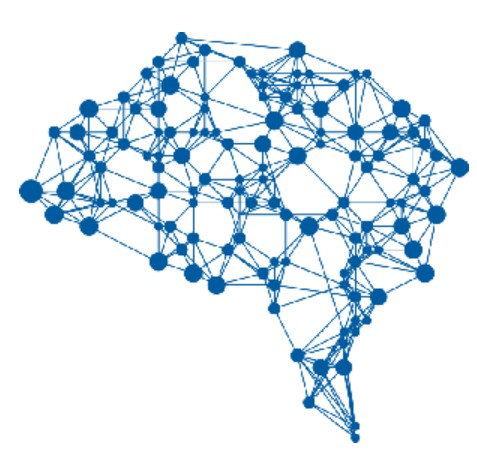
\includegraphics[scale=1]{0.DeepLearningLogo.jpg}
    \end{center}}



\begin{document}
\maketitle
\counterwithin{figure}{subsection}
\captionsetup[figure]{labelfont=bf}

\pagebreak

%% -- Sommario
\tableofcontents
\pagebreak




\section{The 3 Paradigms: Symbolic AI, TML, and Deep Learning}

As a Data Scientist, choosing the right paradigm is as important as understanding the math behind it. Applying Deep Learning to a problem that requires perfect transparency is a failure of system design.

\subsection{Symbolic AI (Rule-Based AI)}

 \begin{defbox}{Symbolic AI}
 Symbolic AI is an approach to artificial intelligence based on high-level human-readable symbols, formal logic, and explicit rules. Knowledge is represented through structures such as logical expressions, symbolic relations, and \texttt{if-then} rules. Reasoning is performed by manipulating these symbolic representations directly.
 \end{defbox}

Symbolic AI is a \textbf{top-down} approach. Instead of learning from data, humans explicitly write the logical rules (if-then statements) that govern the system.

\begin{itemize}
    \item \textbf{Strengths:} Perfect transparency and explainability. It is computationally cheap once the rules are written.
    \item \textbf{Weaknesses:} It is entirely rigid. If the environment changes or the problem is too complex (like recognizing a face in an image), writing all the necessary rules becomes impossible.
    \item \textbf{When to use:} When the problem domain is fully understood, strictly governed by clear rules (e.g., tax calculation software), and 100\% interpretability is legally required.
\end{itemize}

\subsection{Traditional Machine Learning (TML)}
TML is a \textbf{bottom-up} approach where algorithms learn patterns from data rather than explicit programming. 

 \begin{defbox}{Traditional Machine Learning}
 TML is a subset of artificial intelligence in which algorithms learn patterns from data without being explicitly programmed with all decision rules. Instead of manually writing every rule, the system learns predictive relationships from data.
 \end{defbox}

  Some classical TML algorithms.

\begin{itemize}
 \item A \textbf{Decision Tree} is a predictive model that recursively splits the data according to feature-based conditions, producing a tree-like structure of decisions.

 \vs


 \item A \textbf{Support Vector Machine (SVM)} is a supervised learning algorithm that finds a decision boundary, called a hyperplane, that best separates classes in the feature space.

 \vs


\item \textbf{ Linear Regression} is a model used to predict a continuous target variable by assuming a linear relationship between the input features and the output.
 
\vs


\item \textbf{ K-Nearest Neighbors (KNN)} is an algorithm that classifies a sample according to the majority class among its nearest data points in the feature space.
 
\vs


\item \textbf {Random Forest} is an ensemble learning method that combines many decision trees in order to improve predictive accuracy and reduce overfitting.
\end{itemize}

These algorithms are fundamental in Data Mining because they cover both classification and regression tasks, and they are often strong baselines in structured-data problems.

\vspace{-0.2cm}
\paragraph*{The Bottleneck: Feature Engineering.}
TML models (like Random Forests, SVMs, or Linear Regression) generally cannot process complex raw data (like raw pixels or raw audio waves). A human expert must manually perform \textbf{Feature Engineering}: extracting the relevant variables from the raw data before feeding them to the algorithm. 

\begin{itemize}
    \item \textbf{Strengths:} Highly effective on \textbf{Structured Data} (tabular data like Excel sheets). It works well with small-to-medium datasets, trains quickly on standard CPUs, and often remains highly interpretable.
    \item \textbf{Weaknesses:} Performance is entirely dependent on human skill in feature engineering. It struggles heavily with Unstructured Data (images, text, video).
    \item \textbf{When to use:} Business analytics, finance (credit scoring), customer segmentation, and any scenario with tabular data where explainability and low compute cost are priorities.
\end{itemize}

\subsection{Deep Learning (DL)}

Deep Learning is a subset of ML based on deep neural networks. Its defining characteristic is \textbf{Automatic Feature Extraction}.

 \begin{defbox}{Deep Learning}
 Deep Learning is a specialized branch of machine learning based on neural networks with many layers. These models automatically learn hierarchical feature representations from raw data and are especially effective on large and complex datasets.
 \end{defbox}

 The  three major DL architectures are:

\begin{itemize}
 \item A \textbf{Convolutional Neural Network (CNN)} is a neural network architecture especially suited for image data, where local spatial patterns and hierarchical visual features are important.
\vs


\item  A \textbf{Recurrent Neural Network (RNN) }is a neural architecture designed for sequential data, where the order of the elements matters, such as time series or text.
\vs


 \item A \textbf{Transformer} is a neural architecture based on self-attention mechanisms, able to process input elements in parallel and capture long-range dependencies very effectively.

\end{itemize}

CNNs are historically strong in vision, RNNs in sequential modeling, and Transformers are now extremely important in NLP and many other domains.


Instead of a human manually designing features, raw data is fed directly into the network. The early hidden layers learn simple features (like edges in an image), and deeper layers combine them into complex features (like faces).

\begin{itemize}
    \item \textbf{Strengths:} State-of-the-art performance on \textbf{Unstructured Data} (Computer Vision, Natural Language Processing). It completely removes the human feature-engineering bottleneck.
    \item \textbf{Weaknesses:} It requires massive amounts of labeled data to prevent \textbf{overfitting}. It requires expensive hardware (GPUs/TPUs) to train. Most importantly, it acts as a \textbf{Black Box}$\rightarrow$ it is extremely difficult to explain \textit{why} the network made a specific prediction.
    \item \textbf{When to use:} Image recognition, translation, speech-to-text, and generative AI, where data is massive and unstructured, and raw predictive power is more important than perfect transparency.
\end{itemize}



\end{document}